\chapter{Ausarbeitung}
\section{Aufgabe 1: Legendre-Funktionen}
\subsection{a}
Die unnormierten Legendrepolynome
\begin{gather}
	P_3(t) = \frac{2n-1}{n} t P_2(t) - \frac{n-1}{n}P_1(t) = \frac{5}{2}t^3-\frac{3}{2}t \\
	P_4(t) = \frac{2n-1}{n} t P_3(t) - \frac{n-1}{n}P_2(t) = \frac{35}{8}t^4 - \frac{15}{4}t^2 + \frac{3}{8}
\end{gather}
Normierungsfaktoren:
\begin{equation}
	N_{l,0} = \sqrt{(2l+1)}	
\end{equation}
$N_{0,0} = 1$, $N_{1,0} = \sqrt{3}$, $N_{2,0} = \sqrt{5}$, $N_{3,0} = \sqrt{7}$, $N_{4,0} = 3$.
\subsection{b}
Um zu untersuchen, ob auch die zugeordneten Legendrefunktionen immer orthogonal zueinander sind, gilt es das Integral des Produktes der Legendre-Polynome zu untersuchen. Hierbei seien die Integralgrenzen -1 und 1. Ergibt das Integral mit den genannten Grenzen 0, so sind die entsprechneden Legendre-Funktionen orthogonal zueinander. Für die Untersuchung ist es vorweg sinnvoll sich auf diejenigen Polynome, die multipliziert miteinander einen geraden Exponenten erzeugen, zu konzentrieren. Das Produkt erzeugt nämlich anschließend einen ungeraden Exponenten nach der Integration. Bei Einsetzen der Integralgrenzen entstehen folglich unterschiedliche Vorzeichen, welche das gesamte Integral ungleich 0 werden lassen könnten. Nun kann man jegliche Untersuchungen durchführen. Notiert wird jedoch diejenige, die beweist, dass nicht alle Legendre-Funktionen orthogonal zueinander sind. Hierfür prüft man das Integral des Produkts aus $P_{0,0}(t)$ und $P_{2,2}(t)$.

\begin{align}
\int_{-1}^{1} P_{0,0}(t) \cdot P_{2,2}(t) &= \int_{-1}^{1} P_{2,2}(t) \\
&= \int_{-1}^{1} \sqrt{\dfrac{5}{12}(1-t^2)} \\
&= \dfrac{\sqrt{15}}{6} \left[ t- \dfrac{1}{3}t^3 \right]_{-1}^1 \\
&= \dfrac{\sqrt{15}}{6} \left( 1- \dfrac{1}{3} - \left(-1+ \dfrac{1}{3}\right) \right) \\
&= \dfrac{2\sqrt{15}}{9} \neq 0
\end{align}   

Durch die obige Berechnung wurde gezeigt, dass nicht alle Legendrefunktionen immer auch orthogonal zueinander sind. 


\clearpage
\section{Aufgabe 2: Sphärisch-Harmonische Analyse}
\begin{equation}
	Y_{n,m}(t) = P_{n,m}(t) \begin{Bmatrix}
	\sin(m\lambda) \\
	\cos(m \lambda)
	\end{Bmatrix}
\end{equation}
\subsection{a}
Für $f_1$, weil $f_1$ nur von $\theta$ abhängig ist und $\int_{0}^{2\pi}\sin(m\lambda) = 0$, nimmt man hier nur $\cos(m\lambda)$
\begin{equation}
	f_1(\lambda,\theta) = \cos^2\theta \Longrightarrow f_1(\lambda,t) = t^2 
\end{equation}
\begin{align}
	c_{n,m}^{f_1} = & \frac{1}{4\pi} \int_{-1}^{1} \int_{0}^{2\pi} N_{n.m} \cdot P_{n,m}(t) \cdot \cos(m\lambda) \cdot f_1(\lambda,t) d\lambda dt \\
	= & \frac{1}{4\pi} \int_{-1}^{1} N_{n.m} \cdot P_{n,m}(t) \cdot t^2  \left[\int_{0}^{2\pi} \cos(m\lambda) d\lambda\right]  dt
\end{align}
\begin{equation}
	\int_{0}^{2\pi} \cos(m\lambda) d\lambda = \begin{cases}
	0 & m \neq 0 \\
	2\pi & m=0
	\end{cases}
\end{equation}
Wenn $m=0$:
\begin{equation}
	c_{n,0}^{f_1} = \frac{N_{n,0}}{2} \int_{-1}^{1} P_{n,0}(t) \cdot t^2 dt
\end{equation}
Wenn $n$ ungerade ist, ist der Grad von t von $P_{n,0}\cdot t^2$ auch ungerade. Da $\int_{-1}^{1} t^{2n-1}dt = 0$, muss man nur $c_{0,0}^{f_1}$, $c_{2,0}^{f_1}$, $c_{4,0}^{f_1}$ berechnen.
\begin{align}
	& c_{0,0}^{f_1} = \frac{1}{2} \int_{-1}^{1} t^2 dt = \frac{1}{3} \\
	& c_{2,0}^{f_1} = \frac{\sqrt{5}}{2} \int_{-1}^{1} \left(\frac{3}{2}t^2-\frac{1}{2}\right)t^2dt = \frac{2\sqrt{5}}{15} \\
	& c_{4,0}^{f_1} = \frac{3}{2} \int_{-1}^{1} \left(\frac{35}{8}t^4 - \frac{15}{4}t^2 + \frac{3}{8}\right)t^2dt = 0
\end{align}
Für $f_2$, weil:
\begin{align}
	& \int_{0}^{2\pi}\cos(kt)\sin(nt)dt = 0 \\
	& \int_{0}^{2\pi}\sin(kt)\sin(nt)dt = \begin{Bmatrix}
	\pi & \text{für  } k=n \\
	0 &\text{sonst}
	\end{Bmatrix}
\end{align}
Man muss nur $m=1$ für $Y_{n,1} = P_{n,1}\sin(\lambda)$ berechnen. Wenn $n$ gerade ist, ist der Grad von t ungerade. Deshalb sind die Berechnungen nur für $c_{1,1}^{f_2}$ und $c_{3,1}^{f_2}$ notwendig.
\begin{align}
	c_{1,1}^{f_1} = \ & \frac{1}{4\pi}\int_{-1}^{1}\left(\sqrt{1-t^2}\right)^3\sqrt{3}\sqrt{1-t^2}\pi dt\\
	= \ & \frac{\sqrt{3}}{4} \int_{-1}^{1} \left(t^4 - 2t^2 +1\right)dt \\
	= \ & \frac{4\sqrt{3}}{15} \\
	c_{3,1}^{f_2} = \ & \frac{1}{4\pi}\int_{-1}^{1}\left(\sqrt{1-t^2}\right)^3\sqrt{\frac{7}{6}}\cdot \frac{3}{2}\left(5t^2-1\right)\sqrt{1-t^2} \pi dt \\
	= \ & \frac{3}{8}\sqrt{\frac{7}{6}}\int_{-1}^{1}\left(5t^6 - 11t^4 + 7t^2-1\right) dt \\
	= \ & -\frac{4}{35} \sqrt{\frac{7}{6}} \\ 
	= \ & -\frac{2\sqrt{42}}{105}
\end{align}
Für $f_3$:\\
Ähnlich wie für $f_1$, nimmt man nur $\cos(m\lambda)$ und $c_{n,m}^{f3} = 0$ wenn $m \neq 0$. Man benennt:
\begin{equation*}
	J_k = \int_{-1}^{1} t^k \cosh (t) dt
\end{equation*}
Dann:
\begin{align}
	c_{0,0}^{f_3} = \ & \frac{1}{2} \int_{-1}^{1} 1 \cosh (t) dt = \frac{1}{2} J_0 \\
	c_{1,0}^{f_3} = \ & \frac{\sqrt{3}}{2} \int_{-1}^{1} t \cosh (t) dt = \frac{\sqrt{3}}{2}J_1 \\
	c_{2,0}^{f_3} = \ & \frac{\sqrt{5}}{2} \int_{-1}^{1} \left(\frac{3}{2}t^2-\frac{1}{2}\right)\cosh (t) dt = \frac{3\sqrt{5}}{4}J_2-\frac{\sqrt{5}}{4} J_0 \\
	c_{3,0}^{f_3} = \ & \frac{\sqrt{7}}{2} \int_{-1}^{1} \left(\frac{5}{2}t^3 - \frac{3}{2}t\right)\cosh (t) dt = \frac{5\sqrt{7}}{4}J_3 - \frac{3\sqrt{7}}{4} J_1 \\
	c_{4,0}^{f_3} = \ & \frac{3}{2} \int_{-1}^{1} \left(\frac{35}{8}t^4 - \frac{15}{4}t^2 + \frac{3}{8}\right) \cosh (t) dt = \frac{105}{16}J_4 - \frac{45}{8}J_2 + \frac{9}{16}J_0 \\
\end{align}
$J_0$ kann direkt berechnet werden:
\begin{equation}
	J_0 = \int_{-1}^{1} \cosh (t)dt = \left[\sinh(t)\right]^1_{-1} = 2\sinh(1)
\end{equation}
$J_1$ kann via partielle Integration berechnet werden:
\begin{align}
	J_1 & = \int_{-1}^{1} t \cosh(t) dt \\
	 	& = \left[t\sinh(t)\right]^{1}_{-1} - \int_{-1}^{1} \sinh(t) dt \\
	 	& = \left[t\sinh(t)\right]^{1}_{-1} - \left[\cosh(t)\right]^{1}_{-1} \\
	 	& = 0
\end{align}
$J_2$ bis $J_4$ werden via partielle Integration rekursiv berechnet: 
\begin{align}
	J_k = & \int_{-1}^{1} t^k \cosh(t) dt \\
		= & \left[t^k\sinh(t)\right]_{-1}^{1} - \int_{-1}^{1}k t^{k-1} \sinh(t) dt \\
		= & \left[t^k\sinh(t)\right]_{-1}^{1} - k\left[t^{k-1}\cosh(t)\right]_{-1}^{1} + k(k-1)\int_{-1}^{1} \cosh(t)t^{k-2}dt \\
		= & \left[t^k\sinh(t)\right]_{-1}^{1} - k\left[t^{k-1}\cosh(t)\right]_{-1}^{1} + k(k-1)J_{k-2}
\end{align}
Wenn $t$ ungerade ist: $J_k = 0-0+k(k-1)J_{k-2}$. Denn $J_1 = 0$, $J_k = 0$ für alle ungerade $k$. \\\\
Für gerade $k$:
\begin{align}
	J_k = 2\sinh(1) - 2k\cosh(1) + k(k-1)J_{k-2} 
\end{align}
Ansatz:
\begin{align}
	J_2 = \ & 2\sinh(1) - 4\cosh(1) + 2J_0 \\
	= \ & 2\sinh(1) - 4\cosh(1) + 4 \sinh(1) \\
	= \ & 6\sinh(1) - 4\cosh(1) \\
	J_4 = \ & 2\sinh(1) - 8\cosh(1) + 12 J_2\\
		= \ & 2\sinh(1) - 8\cosh(1) + 12 (6\sinh(1) - 4\cosh(1))\\
		= \ & 74 \sinh(1) - 56\cosh(1)
\end{align}
Berechnung von Koeffizienten:
\begin{align}
	c_{0,0}^{f_3} = \ & \sinh(1) \\
	c_{1,0}^{f_3} = \ & 0 \\
	c_{2,0}^{f_3} = \ & 4\sqrt{5}\sinh(1) - 3\sqrt{5} \cosh(1) \\
	c_{3,0}^{f_3} = \ & 0 \\
	c_{4,0}^{f_3} = \ & 453\sinh(1) - 345\cosh(1)
\end{align}
\subsection{b}
Für $f_1$: 
\begin{align}
	\sum_n \sum_m c_{n,m}^{f_1} \bar{Y}_{n,m}(\lambda,t)  = \ & c_{0,0}^{f_1} \bar{Y}_{0,0}(\lambda,t) + c_{2,0}^{f_1} \bar{Y}_{2,0}(\lambda,t) +c_{4,0}^{f_1} \bar{Y}_{4,0}(\lambda,t) \\
	   = \ & \frac{1}{3} \cdot 1 \cdot \cos(0) + \frac{2\sqrt{5}}{15} \cdot \sqrt{5} \cdot (\frac{3}{2}t^2 - \frac{1}{2}) \cdot \cos(0) + 0 \\
	   = \ & t^2 \\
	   = \ & \cos^2(\theta)
\end{align}
Für $f_2$:
\begin{align}
	\sum_n \sum_m c_{n,m}^{f_2} \bar{Y}_{n,m}(\lambda,t) = \ & c_{1,1}^{f_2} \bar{Y}_{1,1}(\lambda,t) + c_{3,1}^{f_2} \bar{Y}_{3,1}(\lambda,t) \\
	= \ & \frac{4\sqrt{3}}{15} \cdot  \sqrt{3} \sqrt{1-t^2} \sin(\lambda) - \frac{2\sqrt{42}}{105} \cdot \sqrt{\frac{7}{6}}\cdot \frac{3}{2}(5t^2-1)\sqrt{1-t^2} \sin(\lambda) \\
	= \ & \frac{3}{4} \sin \theta \sin \lambda - \frac{1}{4} \sin3\theta \sin \lambda
\end{align}
Mit MATLAB ist das maximale Ergebnis von $\frac{3}{4} \sin \theta \sin \lambda - \frac{1}{4} \sin3\theta \sin \lambda - \sin^3(\theta)\sin(\lambda)$ im Bereich von $10^{-16}$ (bis zum $n = m = 4$)\\\\
Für $f_3$:
\begin{align}
	\sum_n \sum_m c_{n,m}^{f_2} \bar{Y}_{n,m}(\lambda,t) = \ & c_{0,0}^{f_3} \bar{Y}_{0,0}(\lambda,t) + c_{2,0}^{f_3} \bar{Y}_{2,0}(\lambda,t) + c_{4,0}^{f_3} \bar{Y}_{4,0}(\lambda,t) \\
	= \ & \sinh(1) + (4\sqrt{5}\sinh(1)-3\sqrt{5}\cosh(1)) \cdot \sqrt{5} \cdot \frac{1}{4}(1+3\cos(2\theta)) \\
	& + (453\sinh(1) - 345\cosh(1)) \cdot 3 \cdot (\frac{35}{8}\cos^4\theta - \frac{15}{4}\cos^2\theta + \frac{3}{8})
\end{align}
Mit MATLAB ist das maximale Ergebnis von $\cosh(\cos \theta) -\sum_n \sum_m c_{n,m}^{f_2} \bar{Y}_{n,m}(\lambda,t) $ im Bereich von $10^{-5}$ (bis zum $n = m = 4$)
\clearpage
\section{Aufgabe 3: Rotation von Kugelflächenfunktionen}
\subsection{Implementierung der Wigner-d-Funktionen $d_{km}^n(\beta)$}
Die zu implementierende (ineffektive) Summendarstellung sieht wie folgt aus: 
\begin{gather}
d_{km}^n(\beta) = \sqrt{\dfrac{(n+m)!(n-m)!}{(n+k)!(n-k)!}} \sum_{t=t_1}^{t_2} \binom{n+k}{t} \binom{n-k}{n-m-t} (-1)^t \left( \cos \dfrac{\beta}{2} \right)^{2n-a} \left( \sin \dfrac{\beta}{2} \right)^a \\
\text{mit} ~~~ a = m-k+2t, ~~~ t_1 = max(0,k-m) ~ \text{und} ~ t_2 = min(n-m, n+k)
\end{gather}
Die Funktion ist auf der nächsten Seite zu sehen oder dem Anhang zu entnehmen. 
\begin{lstlisting}

	function[d] = Wigner_d(m,n,k,beta)
	% Nicholas Schneider & Ziqing Yu
	% 30/11/2020
	% Mit dieser Funktion kann man die Wigner-d-Funktion berechnen. 
	% input: Grad n,
	%        Ordnung m und k
	%        Winkel beta	
	% output: Wigner-d-Funktion

	% pruefen, ob m,n,k ganzzahlig ist
	if (rem(m,1)~=0 || rem(n,1)~=0 || rem(k,1)~=0)
	error('n,m,k muessen ganzzahlig sein.')
	end
	% pruefen, ob -n<=k und m<=n
	if (-n > k || m> n || -n >k || k>n)
	error('Bedingungen -n<=k oder m<=n nicht erfuellt.')
	end
	% SQRT berechnen
	SQRT = sqrt((factorial(n+m) * factorial(n-m)) ...
	/ (factorial(n+k) * factorial(n-k)));
	
	%
	t1 = max(0,k-m);
	t2 = min(n-m,n+k);
	
	Sigma = 0;
	for t = t1:t2
	a = m - k + 2 * t;
	Sigma = Sigma + binomfun(n+k,t) * binomfun(n-k,n-m-t) ...
	* (-1)^t * cos(beta/2)^(2*n-a) * sin(beta/2)^a;
	end
	d = SQRT * Sigma;
	end
\end{lstlisting}
\subsection{Rotation der Kugelflächenfunktionen und Visualisierung}
Mit dem Winkel $\gamma=\frac{\pi}{12}$ soll die Rotation der Kugelflächenfunktion $\hat{Y}_{6,4}$ getestet werden. Dabei soll der Meta-Pol in Stuttgart ($\Lambda = 9^{\circ}11'$, $\Phi = 48^{\circ}46'$) liegen. 
\begin{figure}[H]
\centering
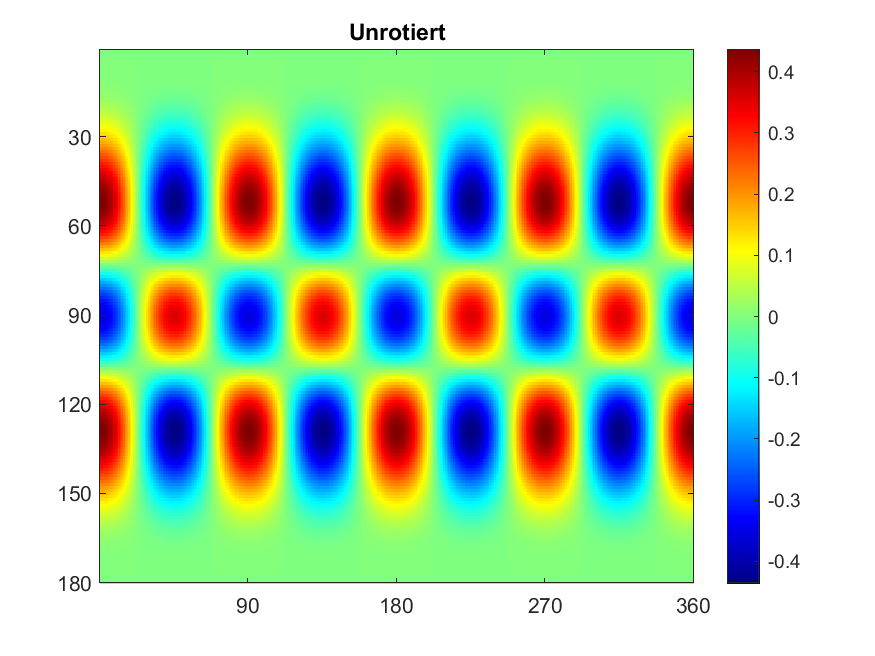
\includegraphics[scale = 0.6]{unrotiert.png}
\caption{Ergebnis der Kugelflächenfunktion unrotiert}
\label{unrot}
\end{figure}
Abbildung \ref{unrot} zeigt zunächst das unrotierte Ergebnis der Kugelflächenfunktion. 
\begin{figure}[H]
	\centering
	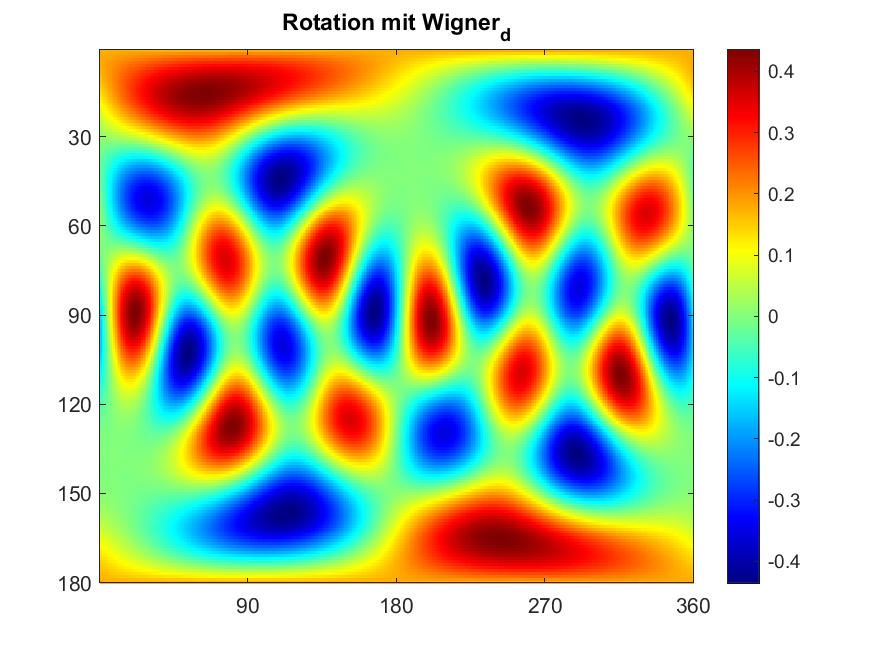
\includegraphics[scale = 0.6]{wigner.png}
	\caption{Rotation der Kugelflächenfunktion über Wigner}
	\label{wigner}
\end{figure}
Abbildung \ref{wigner} präsentiert das Ergebnis der Rotation der Kugelflächenfunktion, die durch die Berechnung über Wigner entstanden ist. 
\begin{figure}[H]
	\centering
	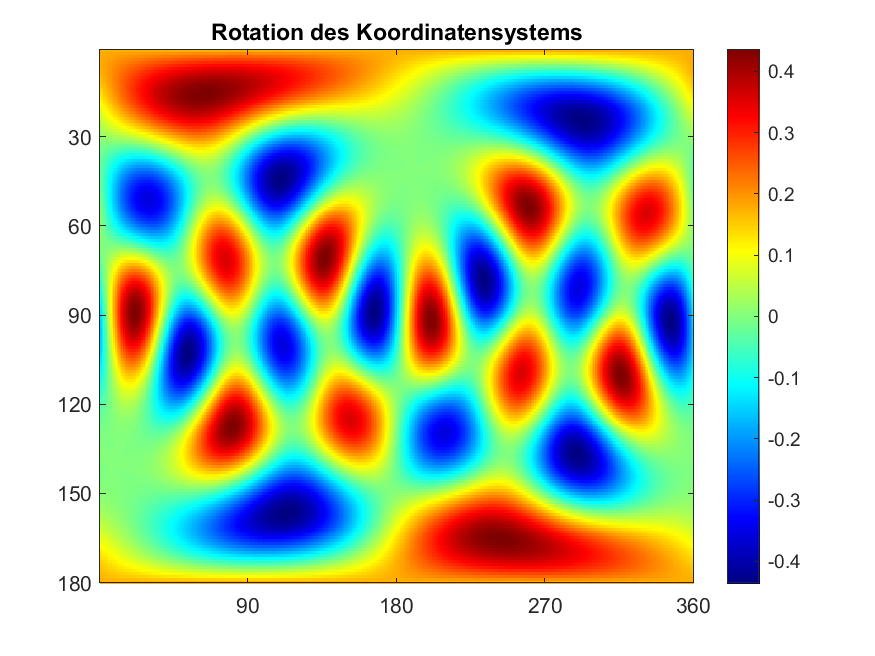
\includegraphics[scale = 0.6]{rotiert.png}
	\caption{Rotation der Kugelflächenfunktion mit Stuttgart als Meta-Pol}
	\label{rot}
\end{figure}
In Abbildung \ref{rot} ist die Rotation der Kugelflächenfunktion mit Stuttgart als Meta-Pol dargestellt. 
\begin{figure}[H]
 	\centering
 	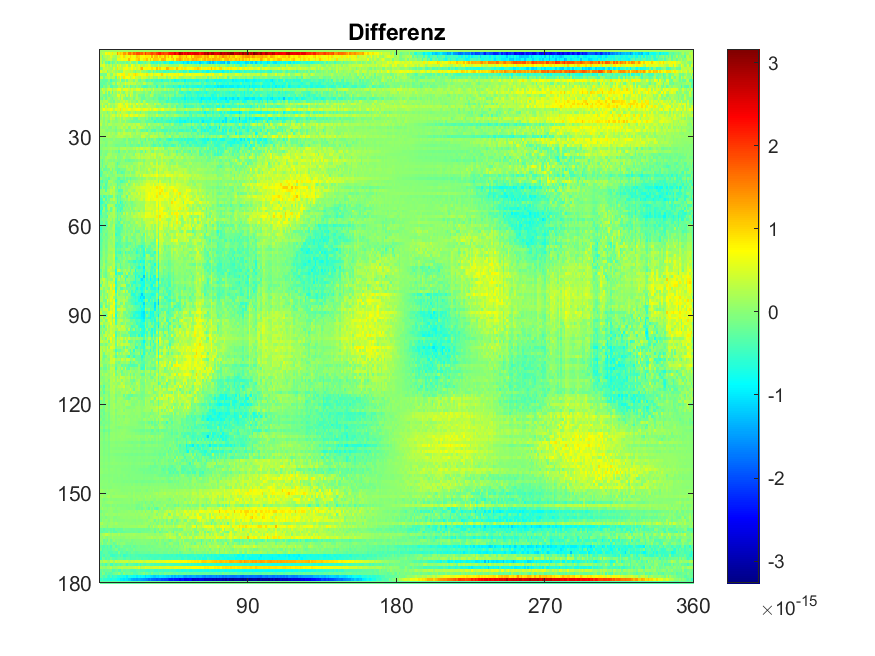
\includegraphics[scale = 0.6]{diff.png}
 	\caption{Differenz beider Berechnungen}
 	\label{diff}
\end{figure}
In Abbildung \ref{diff} sieht man nun den Plot der Differenzen beider Berechnungen. Die maximale Differenzen sind im Bereich von $3 \cdot 10^{-15}$.